\documentclass{article} % For LaTeX2e
\usepackage{nips14submit_e,times}
\usepackage{hyperref}
\usepackage{url}
\usepackage{graphicx}
\usepackage{amsmath}
\usepackage{amssymb}
\usepackage{anyfontsize}
\usepackage{subcaption}
\usepackage{titling}
\usepackage{array}
\usepackage{authblk}

\title{Latent Predicate Networks: Concept Learning with Probabilistic Context-Sensitive Grammars}

\author{Eyal Dechter\thanks{{\tt \{edechter, rule, jbt\} @mit.edu}}}
\author{Joshua Rule}
\author{Joshua B. Tenenbaum}
\affil{Department of Brain and Cognitive Sciences, MIT}

\newcommand{\fix}{\marginpar{FIX}}
\newcommand{\new}{\marginpar{NEW}}

\nipsfinalcopy % Uncomment for camera-ready version

\begin{document}

\maketitle

\begin{abstract}
  For humans, learning abstract concepts and learning language go hand
  in hand: we acquire abstract knowledge primarily through linguistic
  experience, and acquiring abstract concepts is a crucial step in
  learning the meanings of linguistic expressions. Number knowledge is
  a case in point: we largely acquire concepts such as seventy-three
  through linguistic means, and we can only know what the sentence
  ``seventy-three is more than twice as big as thirty-one" means if we
  can grasp the meanings of its component number words. How do we
  begin to solve this problem? One approach is to estimate the
  distribution from which sentences are drawn, and, in doing so, infer
  the latent concepts and relationships that best explain those
  sentences. We present early work on a learning framework called
  Latent Predicate Networks (LPNs) which learns concepts by inferring
  the parameters of probabilistic context-sensitive grammars over
  sentences.  We show that for a small fragment of sentences
  expressing relationships between English number words, we can use
  hierarchical Bayesian inference to learn LPNs that can answer simple
  queries about previously unseen relationships within this
  domain. These generalizations demonstrate LPNs' promise as a tool
  for learning and representing conceptual knowledge in language.
\end{abstract}

\section{Introduction}

Although concept learning and language acquisition have typically been
treated as distinct problems in AI, linguistics and cognitive
development, they are strongly coupled for a child learning to
understand language. More generally, people learn many abstract
concepts primarily through language even though understanding language
depends on understanding the underlying concepts. Research in concept
learning is often focused on concepts grounded in perceptual features,
and while it is almost certainly true that many concepts are learned
via generalization from concrete examples, some concepts cannot be
learned this way.

Number concepts are a good example: children do not learn about the
meaning of ``seventy five'' by seeing examples of seventy five things;
they do not know that ``seventy five'' is more than ``twenty five''
because of their perceptual experiences of these quantities. Rather,
children learn the meaning of ``seventy five'' (or ``a billion and
five'') by noticing how number words are used in language, in counting
sequences, in arithmetic exercises, {\it etc}. Other good examples of such
abstract concepts are kinship and social relations ({\it e.g.} ``my father
in law's grandmother''), temporal relations (``the day after last
Thanksgiving.''), and spatial relations (``above and just to the left
of'').

Such concepts share many of the properties of
language syntax: they are unbounded in number, they derive
their meanings via composition, and, although people only ever say,
hear, or read about a small number of them, they are able to reason
correctly about any them. There seems to be a grammar to these
concepts, and grasping this grammar is critical to understanding their
meanings and how to use them. This motivates our approach here, which
is to apply the tools of probabilistic grammars more familiar from
studies of syntax to the problem of concept aquisition.

Doing so requires overcoming some technical barriers.

First, whereas context-free grammars are suitable for describing large
swathes of language syntax, the grammars of concepts are not
context-free. To address this, we use Range Concatenation Grammars, a
context-sensitive grammar formalism -- one of several developed within
linguistics -- and extend this formalism to a probabilistic model of
sentences. 

Second, the categories of syntax -- the nonterminals of the grammar --
are often assumed to be known to children innately and given to
automated learners by human experts. The categories that underlie
conceptual knowledge, on the other hand, are far more numerous, vary
from domain to domain, and are unlikely to be known to the
learner. This motivates our use of latent predicates that, through
learning, assume the role of a domain's underlying concepts (in the
number domain, these might correspond to the concepts of
successorship, order of magnitude, magnitude comparison, exact
vs. approximate, {\it etc}.).

Finally, inducing probabilistic context-sensitive grammars with latent
predicates threatens to be intractable: our goal is to find a
middle ground between expressivity and tractability. Using
PRISM~\cite{DBLP:journals/jair/SatoK01} -- a probabilistic logic programming system that naturally
implements efficient dynamic programming algorithms for our models --
we are able to explore which domains and which grammar architectures
are a good fit for this grammar-based approach.

The rest of this paper describes early work on this approach. First,
we present Latent Predicate Networks (LPNs), our probabilistic model
of concept learning. Then, we describe our approach to inference and
its implementation in PRISM. Finally, we present preliminary
experimental results in the domain of number concept learning that
demonstrate the promise of this approach.

\section{Latent Predicate Networks}

\begin{figure}[t]
  \begin{subfigure}[b]{0.5\linewidth}
    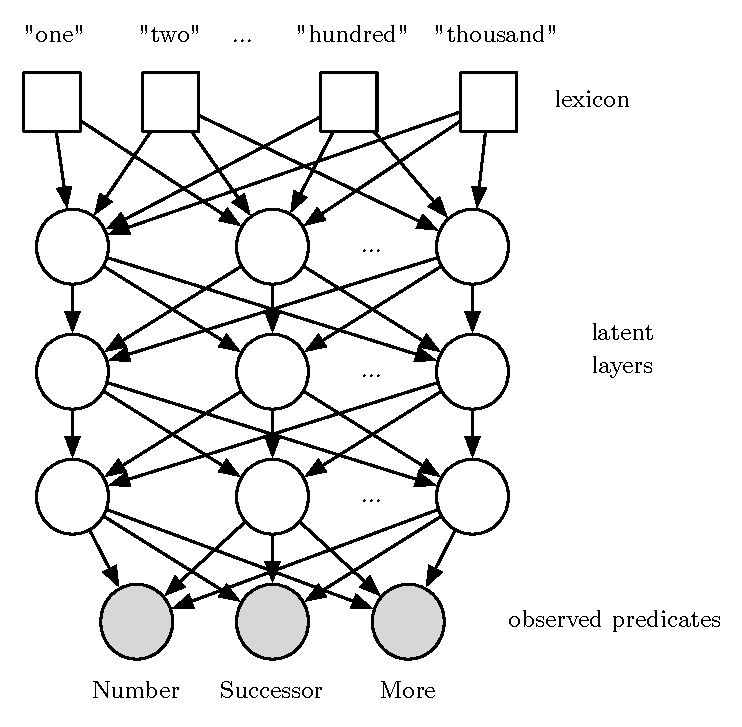
\includegraphics[width=\linewidth]{lpn/lpn.pdf}
    \caption{The architecture and rules of a schematic LPN.}
    \label{fig:architecture}
  \end{subfigure}
  \hfill
  \begin{subfigure}[b]{0.5\linewidth}
    \includegraphics[width=\linewidth]{parseTree/parse.pdf}
    \caption{A possible parse of the sentence ``after twenty five comes twenty six" using a 5-predicate LPN.}
    \label{fig:parseexample}
  \end{subfigure}
\end{figure}

An LPN is a hierarchical Bayesian model of strings
extending the Hierarchical Dirichlet PCFG model (HD-PCFG) to
Probabilistic Range Concatenation Grammars (PRCGs). 

\subsection{Probabilistic Range Concatenation Grammars}
Range Concatenation Grammars (RCGs) are a class of string grammars
that represent all and only those languages that can be parsed in time
polynomial in the length of the target
string~\cite{boullier2005range}. An RCG $G=(N, T, V, P, S)$ is a
5-tuple where $N$ is a finite set of predicate symbols, $T$ is a set
of terminal symbols, $V$ is a set of variable symbols, P is a finite
set of $M \geq 0$ clauses of the form $\psi_0 \rightarrow \psi_1 \dots
\psi_M$, and $S \in N$ is the \emph{axiom}. Each $\psi_m$ is a term of
the form $A(\alpha_1, \dots, \alpha_{\mathcal{A}(A)}$, where $A \in
N$, $\mathcal{A}(A)$ is the arity of $A$, and each $\alpha_i \in (T
\cup V)^*$ is an argument of $\psi_m$. We call the left hand side term
of any clause the \emph{head} of that clause and its predicate symbol
is the \emph{head predicate}.

A string $x$ is in the language defined by an RCG if one can
\emph{derive} $S(x)$. A derivation is a sequence of rewrite steps in
which substrings of the left hand side argument string are bound to
the variables of the head of some clause, thus determining the
arguments in the clause body. If a clause has no body terms, then its
head is derived; otherwise, its head is derived if its body clauses
are derived.\footnote{This description of the language of an RCG
  technically only holds for \emph{non-combinatory} RCGs, in which the
  arguments of body terms can only contain single variables. Since any
  \emph{combinatory} RCG can be converted into a non-combinatory RCG
  and we only consider non-combinatory RCGs here, this description
  suffices.}

We extend RCGs to PRCGs by annotating each clause $C_k \in P$ with
probabilities $p_k$ such that for all predicates ${A \in N, \,
  \sum_{k:head(C_k)=A} p_k = 1}$. A PRCG defines a distribution over
strings $x$ by sampling from derivations of $S(x)$ according to the
product of probabilities of clauses used in that derivation. This is a
well defined distribution as long as no probability mass is placed on
derivations of infinite length; in this paper, we only consider PRCGs
with derivations of finite length, so we need not worry about this
requirement. See Figure \ref{fig:grammar} for an example of the context-sensitive 2-copy language $\{ww\,|w \in \{a,b\}^+\}$ as a PRCG.

\subsection{Generic Architecture}

An LPN is a PRCG with the following generic architecture: the
\emph{axiom} of an LPN is a unary predicate $S$, and it has $K$
densely connected binary predicates $\{A_k\}_{k=1}^K$ (Figure
\ref{fig:architecture}). For each latent predicate $A_k$, we define
rules such that $A_k(w_a,w_b)$ is true for each possible pair of
terminals, $w_a,w_b \in T$. $T$ may include the empty string $\epsilon$, but we
do not allow latent predicates of the form $A_k(\epsilon, \epsilon)$:
see Section~\ref{sec:implementation}. We also define rules such that
$A_k(XY,UV)$ is true for each possible pair of predicates, $A_i,A_j$,
and every possible ordering of the variables $X,Y,U$ and $V$ across
$A_i$ and $A_j$. Finally, we define $S(XY)$ to be the concatenation of
the two arguments of $A_1(X,Y)$.

\subsection{Learning Model}

Given a collection of predicates, $\{A_k\}_{k=1}^{K}$, and a
distribution over clauses, $\{\vec{w}_{A_k}\}$, the learning task is
to model a set of utterances, $\{x_j\}_{j=1}^{J}$, as being generated
according to the following distribution:

\begin{align*}
  \vec{w}_{A_k} &\sim Dir(\vec{\alpha}_{A_k})\\
  x_j &\underset{iid}{\sim} p_{\text{\textsc{prcg}}}(S(x_j)\,|\,\{w_{A_k}\})\\
  p(\{\vec{w}_{A_k}\}\,|\, \vec{x}, \{\vec{\alpha}_{A_k}\}) &\propto
  \prod_j p_{\text{\textsc{prcg}}}(x_j|\{\vec{w}_{A_k}\}) \prod_{A_k}
  p_{\text{\textsc{dir}}}(\vec{w}_{A_k}\,|\,\vec{\alpha}_{A_k})
\end{align*}


In words, the weights of clauses sharing head predicate $A_k$ are
drawn from a Dirichlet distribution defined by
$\vec{\alpha}_{A_k}$. Sentences $x_j$ are then drawn from the
resulting PRCG.

Bayesian inference over stochastic grammars
and stochastic logic programs has been an active area of
research in recent decades~\cite{DBLP:journals/etai/Muggleton00, cussens2001parameter, DBLP:conf/emnlp/LiangPJK07,
  goldwater2006contextual, johnson2006adaptor}.
Variational inference is a popular approach in this domain and the one
we adopt here. As explained in the next section, we implemented
inference by translating LPNs into PRISM programs and using its
built-in Variational Bayes Expectation-Maximization
algorithm~\cite{sato2008variational}. 

\section{Implementation \label{sec:implementation}}

\begin{figure}[t]
	\centering
	\begin{minipage}[b]{0.8\linewidth}
1) A(a, a) :: 0.25. \\
2) A(b, b) :: 0.3. \\
3) A(X a, Y a) $\leftarrow$ A(X, Y) :: 0.25. \\
4) A(X b, Y b) $\leftarrow$ A(X, Y) :: 0.2.
		\subcaption{}
		\label{fig:grammar}
	\end{minipage}
	%\rule[0pt]{0.8\linewidth}{.5pt}
	\begin{minipage}[b]{0.8\linewidth}
        \fontsize{9}{10.5}\selectfont\ttfamily
		\begin{verbatim}
values(`A', [1, 2, 3, 4],
    [0.25, 0.30, 0.25, 0.20]).

reduce(`A'-[[a],[a]],1).
reduce(`A'-[[b],[b]],2).
reduce(`A'-[A2,B2],3) :- lpn(`A'-[X,Y]),
    append(X,[a],A2), append(Y,[a],B2).
reduce(`A'-[A2,B2],4) :- lpn(`A'-[X,Y]),
    append(X,[b],A2), append(Y,[b],B2).

lpn(P-IN) :- reduce(P-IN,V), msw(P,V).
		\end{verbatim}
		\subcaption{}
		\label{fig:prism}
	\end{minipage}
	\caption{Possible encodings of the 2-copy language $\{ww\,|\, w \in \{a,b\}^+\}$ as (\subref{fig:grammar}) an LPN, (\subref{fig:prism}) a PRISM program.}
	\label{fig:copy}
\end{figure}

LPNs can be encoded as a restricted subclass of PRISM programs; this
is very similar to how PCFGs are encoded in
PRISM~\cite{DBLP:conf/cl/2000}. See Figure~\ref{fig:copy} for an
example. A general probabilistic logic programming system based on
PROLOG, PRISM provides built-in predicates for probabilistic execution
and Bayesian inference over logic programs with stochastic
choices. There are several restrictions placed on PRISM programs to
maintain the validity of their probabilistic interpretation. Most
importantly, derivations of a probabilistic predicate cannot contain
cycles. Because we disallow $A_i(\epsilon,\epsilon)$ as a valid
clause, every term in the body of a clause has shorter arguments than
the head, giving acyclic and finite derivations.

\section{Experiment}

To evaluate LPNs as a probabilistic model of concept acquisition, we
trained an LPN with $4$ latent predicates on a set of sentences
expressing successor and predecessor relations in numbers between one
and ninety-nine. The training set was the collection of sentences $$X
= \{[\text{after}\, | \, \text{before}] \, \langle n \rangle \,
\text{comes} \, \langle n+1 \rangle \,|\, n \in 1,\dots,99\},$$ where
$\langle n \rangle$ is the number word corresponding to $n$. The
lexicon was the set of number word corresponding to $1$ through $19$,
the decades $20, \dots, 30$, the empty string, and the words
``before'' and ``after.'' It is not difficult to manually work out an
LPN that describes this limited domain of sentences; see
Figure~\ref{fig:parseexample}, for a possible LPN derivation of an
example sentence.

Although it is difficult to know how common these kinds of sentences
are in child-directed speech, words for small numbers are far more
common than words for larger ones \cite{macwhinney2000childes}. On the
other hand, children learning to count to large numbers rehearse the
sequence. To approximate this distribution of evidence, we drew these
sample sentences from a sum of a geometric distribution with parameter
$0.5$ and a uniform distribution. These components were weighted
$75\%$ and $25\%$, respectively. We drew $2000$ examples from this
distribution, holding out the sentences in Table~\ref{tab:results} for
evaluation.

For inference, we used default $\frac{1}{D}$ pseudocounts (where $D$ is the
dimensionality of the Dirichlet distributions). We found that different random
initialization for this experiment did not lead to qualitatively different
results, though further investigation will be necessary to see how
robust the algorithm is to local maxima when fitting LPNs.

We evaluated the learned model by asking for Viterbi ({\it i.e.} maximum a
posteriori) completions of the last words of each held out test
sentence. Table~\ref{tab:results} shows these completions. The grammar
correctly learns much of the structure of these sentences, including
the difference between sentences starting with ``before'' and
``after'' and the edge cases that relate decade words like ``twenty''
to non-decade words like ``twenty one.''

\begin{table}[h]
  \begin{subtable}[b]{0.5\linewidth}
    \begin{tabular}{>{\tiny} l >{\tiny} l}
      \multicolumn{2}{>{\tiny}c}{$S$(X Y) $\leftarrow$ $A_1$(X, Y) : 1.0000} \\
      \multicolumn{2}{>{\tiny}c}{$A_1$(X Y, U V) $\leftarrow$ $A_2$(X, U), $A_3$(V, Y) : 0.5002} \\
      \multicolumn{2}{>{\tiny}c}{$A_1$(X Y, U V) $\leftarrow$ $A_3$(Y, V), $A_4$(X, U) : 0.3428} \\
      \multicolumn{2}{>{\tiny}c}{$A_1$(X Y, U V) $\leftarrow$ $A_1$(V, Y), $A_4$(X, U) : 0.0796} \\
      \multicolumn{2}{>{\tiny}c}{$A_1$(X Y, U V) $\leftarrow$ $A_1$(Y, V), $A_2$(X, U) : 0.0712} \\
      \multicolumn{2}{>{\tiny}c}{$A_1$(X Y, U V) $\leftarrow$ $A_2$(Y, X), $A_3$(V, U) : 0.0021} \\
      \multicolumn{2}{>{\tiny}c}{$A_1$(X Y, U V) $\leftarrow$ $A_1$(V, Y), $A_2$(X, U) : 0.0013} \\
      \multicolumn{2}{>{\tiny}c}{$A_1$(X Y, U V) $\leftarrow$ $A_2$(V, X), $A_3$(Y, U) : 0.0008} \\
      \multicolumn{2}{>{\tiny}c}{$A_1$(X Y, U V) $\leftarrow$ $A_1$(X, U), $A_2$(V, Y) : 0.0008} \\
      \multicolumn{2}{>{\tiny}c}{$A_1$(X Y, U V) $\leftarrow$ $A_1$(X, U), $A_2$(Y, V) : 0.0008} \\
      \multicolumn{2}{>{\tiny}c}{$A_1$(X Y, U V) $\leftarrow$ $A_1$(X, U), $A_4$(Y, V) : 0.0004} \\
      $A_2$(before, comes) : 0.7316 & $A_4$(after, comes) : 0.9990  \\
      $A_3$(one, two) : 0.3993 &
      $A_3$(two, three) : 0.2063 \\
      $A_3$(three, four) : 0.1093 &
      $A_3$(four, five) : 0.0734 \\
      $A_3$(five, six) : 0.0502 &
      $A_3$(six, seven) : 0.0355 \\
      $A_3$(eight, nine) : 0.0290 &
      $A_3$(seven, eight) : 0.0271 \\
      $A_2$(fifty, fifty) : 0.0375 &
      $A_2$(thirty, thirty) : 0.0361 \\
      $A_2$(eighty, eighty) : 0.0339 &
      $A_3$(null, one) : 0.0231 \\
      $A_2$(forty, forty) : 0.0332 &
      $A_2$(twenty, twenty) : 0.0310 \\
      $A_2$(seventy, seventy) : 0.0296 &
      $A_2$(sixty, sixty) : 0.0274 \\
      $A_2$(ninety, ninety) : 0.0260 &
      $A_3$(eighteen, nineteen) : 0.0064 \\
      $A_3$(sixteen, seventeen) : 0.0049 &
      $A_3$(eleven, twelve) : 0.0044 \\
      $A_3$(nine, ten) : 0.0044 &
      $A_3$(thirteen, fourteen) : 0.0044 \\
      $A_3$(fourteen, fifteen) : 0.0039 &
      $A_3$(ten, eleven) : 0.0034 \\
      $A_2$(null, fifty) : 0.0043 &
      $A_3$(eighty, null) : 0.0030 \\
      $A_3$(seventeen, eighteen) : 0.0030 &
      $A_3$(nine, sixty) : 0.0025 \\
      $A_2$(nine, seventy) : 0.0029 &
      $A_3$(nine, forty) : 0.0020 \\
      $A_2$(null, thirty) : 0.0022 &
      $A_2$(nine, ninety) : 0.0022 \\
      $A_3$(twelve, thirteen) : 0.0015 &
      $A_3$(fifteen, sixteen) : 0.0015 \\
      $A_3$(null, comes) : 0.0010 &
      $A_2$(twenty, after) : 0.0014 \\
      $A_2$(sixty, before) : 0.0007 &
      $A_3$(nineteen, comes) : 0.0005 \\
      $A_4$(nine, thirty) : 0.0010 & \\
    \end{tabular}
    \caption{The 4 predicate LPN trained to model sentences in the number domain. Rules with insignificant weights are removed. This LPN generates the completions in Table \ref{tab:results}.}
    \label{tab:grammar}
  \end{subtable}
  \begin{subtable}[b]{0.5\linewidth}
    \begin{tabular}{>{\footnotesize} l >{\footnotesize} l}
      Question & $K=4$ \\ \hline
      after twenty comes \underline{\hspace{1cm}}? & twenty one \checkmark \\
      after forty five comes \underline{\hspace{1cm}}? & forty six \checkmark \\
      after forty seven comes \underline{\hspace{1cm}}? & forty eight  \checkmark \\
      after forty nine comes \underline{\hspace{1cm}}? & forty ten $\times$ \\
      after fifty nine comes \underline{\hspace{1cm}}? & fifty ten $\times$ \\
      after sixty one comes \underline{\hspace{1cm}}? & sixty two \checkmark \\
      after sixty three comes \underline{\hspace{1cm}}? & sixty four \checkmark \\
      after sixty four comes \underline{\hspace{1cm}}? & sixty five \checkmark \\
      after sixty five comes \underline{\hspace{1cm}}? & sixty six \checkmark \\
      after sixty nine comes \underline{\hspace{1cm}}? & sixty ten $\times$ \\
      after seventy three comes \underline{\hspace{1cm}}? & seventy four \checkmark \\
      after seventy nine comes \underline{\hspace{1cm}}? & seventy ten $\times$ \\
      after ninety five comes \underline{\hspace{1cm}}? & ninety six \checkmark \\
      before twenty three comes \underline{\hspace{1cm}}? & twenty two \checkmark \\
      before thirty comes \underline{\hspace{1cm}}? & thirty eighty $\times$ \\
      before thirty eight comes \underline{\hspace{1cm}}? & thirty seven \checkmark \\
      before forty one comes \underline{\hspace{1cm}}? & forty \checkmark \\
      before fifty three comes \underline{\hspace{1cm}}? & fifty two \checkmark \\
      before sixty eight comes \underline{\hspace{1cm}}? & sixty seven \checkmark \\
      before seventy two comes \underline{\hspace{1cm}}? & seventy one \checkmark \\
      before seventy three comes \underline{\hspace{1cm}}? & seventy two \checkmark \\
      before eighty five comes \underline{\hspace{1cm}}? & eighty four \checkmark \\
      before ninety two comes \underline{\hspace{1cm}}? & ninety one \checkmark \\
      before ninety three comes \underline{\hspace{1cm}}? & ninety two \checkmark \\
      before ninety five comes \underline{\hspace{1cm}}? &ninety four \checkmark \\
    \end{tabular}
    \caption{Viterbi completions of held-out sentences to evaluate an LPN with 4 latent predicates in the number domain.}
    \label{tab:results}
  \end{subtable}
\end{table}

To inspect visually the learned grammar, we thresholded rules
according to the expected number of times they were used in parsing
the training dataset. Table~\ref{tab:grammar} shows all rules with
expected count above $1e-6$. This reduces from $2669$ to $52$ the
number of significant rules. On inspection, predicate $A_2$ forms
``before'' sentences, predicate $A_4$ forms ``after'' sentences,
predicate $A_3$ is successorship recursively defined over the decades
and ones, and predicate $A_2$ is a category for the decade words.

Our LPN does not learn to how to transition between the last word in a decade
and the next decade (e.g. ``seventy nine'' to ``eighty''). Instead, it
makes the intuitively reasonable generalization that ``seventy nine''
should be followed by ``seventy ten.'' 

\section{Discussion}

Though simple, the knowledge learned by LPNs in the number
domain we explore in this paper goes beyond the expressive capacity of
PCFGs and HMMs, and yet it avoids intractability by using a restricted
formalism. The human ability to learn abstract concepts must also rely
on such a compromise, and it remains to be seen to what extent LPNs
can model this ability.

This work leaves many open questions. What domains of concepts are
amenable to being represented and learned by LPNs? Can multiple and
varied systems of concepts be learned at once? Perhaps most
importantly, are there generic architectures for LPNs that allow a
larger number of predicates without an insurmountable blow-up in the
number of rules? One idea which we are pursuing is using layered
connectivity, much like neural networks, to limit the number of rules
in which each predicate participates. 

Many of the algorithms and formalisms used here were originally
developed for use in other closely related areas, including logic
programming and semantic parsing. Semantic parsing, in particular,
seems especially related to the challenge we face here of jointly
learning meaning and structure from
sentences~\cite{berant2013semantic, liang2013learning, kwiatkowski2010inducing, poon2009unsupervised}. Semantic parsing,
however, tends to frame this challenge slightly differently than we do
here, namely, by asking how utterances can be mapped to an explicit
internal logical language. By contrast, we focus here on systems where
meaning and structure seem inseparable. Understanding how these two
approaches relate and inform one another is an interesting and open
question.

\subsubsection*{Acknowledgments}

We should probably include acknowledgments for this paper.

\subsubsection*{References}

\bibliographystyle{amsplain}
\bibliography{nips_workshop}

\end{document}